\chapter{Modulation}
\lit{«Modulationsverfahren zur Sprachübertragung» von Florian B. Wörter (\href{http://www.woerter.at/dud/stuff/modulationsverfahren.pdf}{PDF})}
\lit{Formeln zu AM, FM und PM: Formelsammlung}
Ganz am Anfang hat man grundsätzlich ein Signal im Basisband. Das kann sowohl ein Sprach- als auch ein digitales Signal sein, mit Frequenzen zwischen 0 und 30 kHz (für Satelliten werden noch höhere verwendet, bei der Sprachübertragung geht man im Amateurfunk meist nur bis 3 kHz). In den folgenden Grafiken wird ein Sprachsignal amplitudenmoduliert.

Das Sprachsignal befindet sich zunächst im Basisband stellt das USB dar. Das LSB existiert noch nicht, da es negative Frequenzen in der Praxis nicht gibt.

\begin{figure}[h<!]
 \centering
 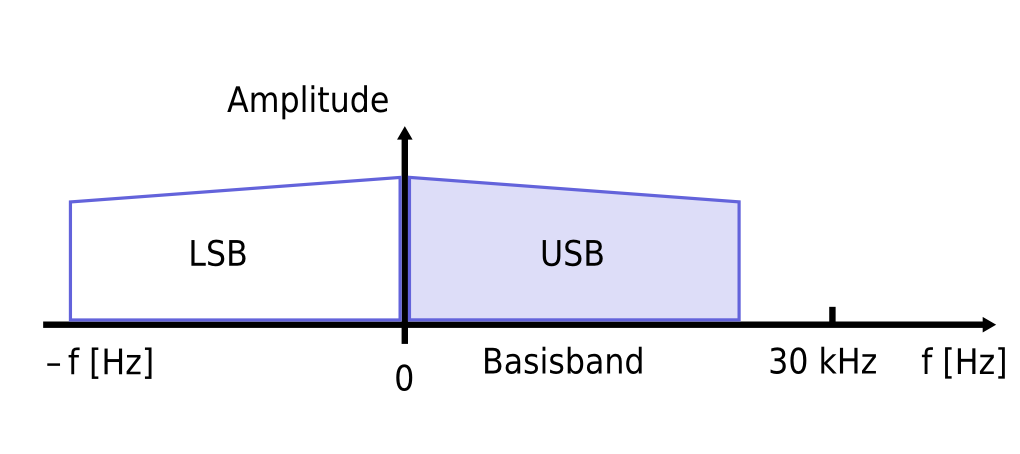
\includegraphics[width=8cm]{./png/Amfu-Modulation-Basisband.png}
 \label{fig:basisband}
\end{figure}


Nun nimmt man eine hochfrequente Trägerschwingung zur Hilfe. Das Signal wird auf sie aufgeprägt (zum Beispiel amplitudenmoduliert), indem man gewisse Eigenschaften (je nachdem die Amplitude, Frequenz oder Phase) der Trägerschwingung proportional zum Signal verändert. So wird das Basisband in den gewünschten Hochfrequenzkanal verschoben.

\begin{figure}[h!]
 \centering
 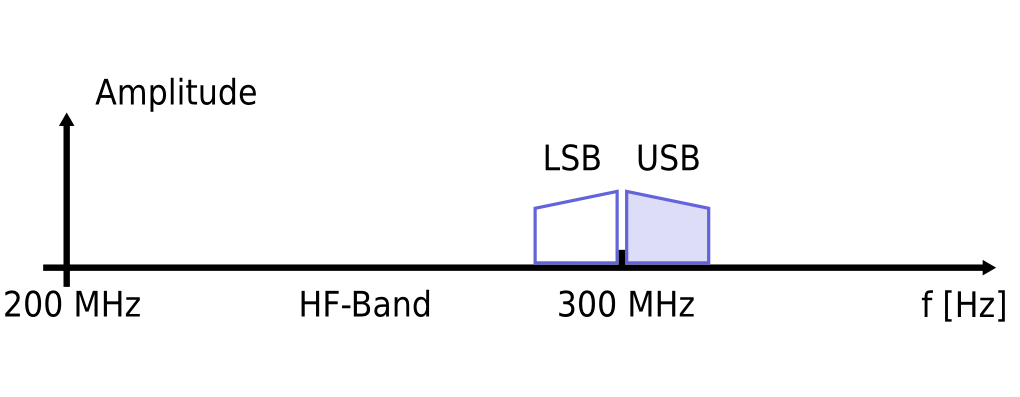
\includegraphics[width=8cm]{./png/Amfu-Modulation-HF.png}
 \label{fig:hfband}
\end{figure}


Während der Amplitudenmodulation wird noch das LSB erzeugt, und es entsteht das Doppelseitenband, das die zweifache NF-Bandbreite aufweist. Da das LSB eine Spiegelung ist, ist es jedoch unnötig und wird etwa bei SSB herausgefiltert.

Man unterscheidet zwischen analogen und digitalen Signalen. Digitale Signale sind zeitdiskret, es wird zwischen festgelegten Zuständen (wie 0/1) gewechselt. Analoge Signale sind zeitkontinuierlich. 

\section{Analoge Modulation}

\subsection{AM}
Bei der Amplitudenmodulation wird auf die Amplitude eingewirkt. Im Frequenzsprektrum wird der Träger als Peak und die beiden Seitenbänder – die die selben Informationen enthalten – sichtbar. Auf dem Träger liegt der grösste Teil der Leistung. Der maximale Wirkungsgrad beträgt (bei einem Modulationsgrad von 1) 17 \%.

\begin{figure}[h!]
 \centering
 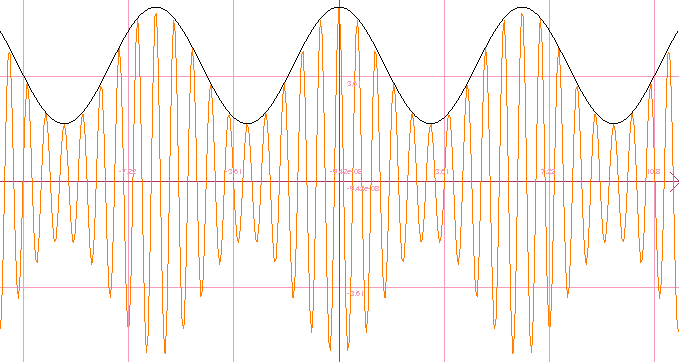
\includegraphics[width=8cm]{./png/Graph_AM.png}
 \caption{Amplitudenmodulation, vereinfacht dargestellt. Das (verschobene) Signal ist schwarz, der Träger orange dargestellt.}
 \label{fig:am}
\end{figure}

Der Modulationsgrad eines AM-Signals ist definiert als das Verhältnis der Amplitude des Signals zur Amplitude des Trägers:

\[
 m = \frac{S_M}{S_T}
\]


Ist der Modulationsgrad grösser als eins, wird das Signal übermoduliert und es treten Verzerrungen auf. 

AM wird von den meisten Rundfunksendern im HF-Band verwendet.

\begin{figure}[h!]
 \centering
 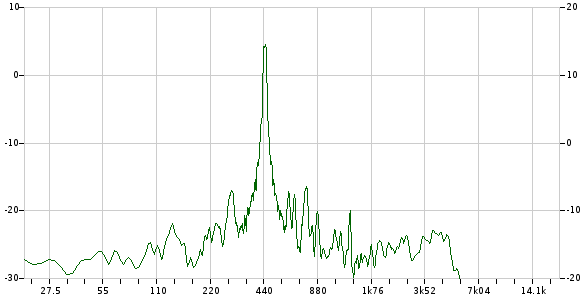
\includegraphics[width=8cm]{./png/AM-Analysis.png}
 \caption{AM-Signal mit dem typischen Peak des Trägersignals}
 \label{fig:amAnalysis}
\end{figure}

Die meisten modernen Amateurfunkgeräte bieten immer noch die Amplitudenmodulation an. Die Aufbereitung der AM geschieht jedoch schon in den Vorstufen des Sendeteils, daher ist die Leistung in der Regel auf 25 \% gegenüber LSB/USB reduziert, um die Endstufe nicht zu überlasten und auch die Linearität zu gewährleisten.

In «echten» AM-Sendern wurde die Modulation bei der Endstufe selbst vorgenommen, und diese konnte im C-Betrieb mit wesentlich grösserer Leistung arbeiten. Dieser scheinbare Vorteil ändert aber nichts an der schlechten Energieeffizienz von AM gegenüber SSB.

AM wird im Amateurfunk kaum noch verwendet. Es gibt noch einige AM-Runden im 80m-Band von OMs, die alte Geräte restaurieren und auch betreiben. Auch im 10m-Band bei 29 MHz sind meist amerikanische OMs in AM aktiv (dort spricht man von «Wintage-Radios»).

Im kommerziellen und auch militärischen Flugfunkverkehr im VHF- und UHF-Bereich wird nach wie vor AM verwendet. Der Grund dafür ist vor allem die Beibehaltung einer Kompatibilität mit älteren Ausrüstungen. Ein weiterer Grund ist die Gewährleistung der Verständlichkeit, wenn z. B. zwei Benutzer gleichzeitig sprechen; dies würde mit FM nicht so sein und könnte zu fatalen Missverständnissen führen. Auf Kurzwelle wir der Flugfunk in USB betrieben, allerdings in einem festen Kanalraster in kHz-Schritten.

Im CB-Funk wurde lange Zeit nur AM gesendet und das Kanalraster entsprechend in 10-kHz-Schritten ausgelegt. Heute wird da vorwiegend in FM im gleichen Kanalraster gearbeitet, oder aber auch in SSB mit Umschaltung LSB/USB. Im «illegalen» CB-Bereich oberhalb 27 405 kHz wird vorwiegend in USB mit 5-kHz-Raster gearbeitet.

\subsection{FM}
Bei der Frequenzmodulation wird auf die Frequenz eingewirkt. Hier wird die Frequenz selber moduliert, was das Signal relativ unanfällig gegenüber Störungen der Amplitude (wie kurze Signalstärkenschwankungen) macht. Mit FM werden die meisten heutigen Radiosendungen moduliert, wie auch Funk auf VHF/UHF.

\begin{figure}[h!]
 \centering
 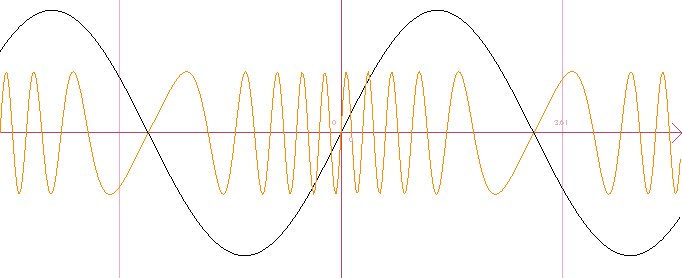
\includegraphics[width=8cm]{./png/Graph_FM.png}
 \caption{Vereinfachte Darstellung von Frequenzmodulation. Das Signal ist schwarz, der Träger orange dargestellt}
 \label{fig:fm}
\end{figure}

Bei FM gewinnt immer das stärkere Signal, d. h. wenn zwei Stationen auf der selben Frequenz senden, hört man den schwächeren nicht. Bei ähnlicher Signalstärke stören sie sich gegenseitig, und man versteht gar nichts. Deshalb wird im Flugfunk auch immer noch AM verwendet.

\begin{figure}[h!]
 \centering
 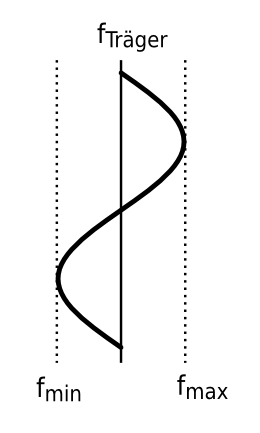
\includegraphics[width=3cm]{./png/Amfu-FM-Wasserfall.png}
 \caption{Sinusförmiges Signal, dieses Mal in der Wasserfalldarstellung. Hier wird die ursprüngliche Signalform wieder sichtbar.}
 \label{fig:fmWaterfall}
\end{figure}

Auf HF kann man mit modernen Transceivern zwar FM senden, was prinzipiell nach dem FMG auch erlaubt wäre. In den Bandplänen, die von den Amateuren selbst ausgearbeitet wurden, ist das jedoch nicht vorgesehen. Einzig im 10m-Band oberhalb etwa 29.5 MHz wird exklusiv in FM gearbeitet, und es gibt dort auch Relais-Stationen mit 100 kHz Abstand zwischen RX und TX (z. B. Relais hb9hd auf 29 660 kHz TX bzw. 29 560 kHz RX).

\subsection{SSB}
Single Side Band; hier wird nur das untere (Lower Side Band, LSB) bzw. das obere Seitenband (Upper Side Band, USB) verwendet, was mit 2.7 kHz (\link{NF-Bandbreite}) weniger als der Hälfte der von AM benötigten Bandbreite entspricht. Da zudem auch der Träger herausgefiltert wird, benötigt man so nur einen Sechstel der Leistung, die für AM notwendig wäre.

Unterhalb von 10 MHz wird meist LSB verwendet, darüber USB.

SSB findet bevorzugt auf dem HF-Frequenzband Verwendung.

\section{Digitale Modulation}
Seit einigen Jahren wird auch für Sprechfunk vermehrt digitale Modulation (vor allem QPSK) erprobt und auch angewendet. Hier wird das analoge Sprachsignal abgetastet und so digital codiert. Danach steht ein digitaler Datenstrom zur Verfügung. Dies ermöglicht auch weltweites Routing übers Internet. Es scheint, dass sich der D-Star-Standard von Icom diesbezüglich durchsetzt.

Heute dominieren sogenannte OFDM-Verfahren, wo innerhalb eines Kanals eine Vielzahl von PSK-, QPSK- oder QAM-modulierte Träger übertragen werden, auf denen dann die erforderlichen Biströme verteilt sind. Ein Beispiel ist DRM auf KW/MW-Rundfunk. 

Die Vorteile sind eine klare Modulation wie in FM, eine relative Unempfindlichkeit gegen Verzerrungen durch die Ionosphäre und ein sauberes Spektrum. Es ist damit auch möglich, Standbilder oder grössere Datenmengen zu übertragen. Diese Verfahren werden durch einen PC oder von Standalone-Geräten (z. B. von AOR), die an die Mike- und NF-Buchsen angeschlossen werden, erzeugt und demoduliert.

\subsection{ASK}
Das \textit{Amplitude Shift Keying} (Amplitudenumtastung) wird für digitale Übertragungen nur noch selten verwendet. Der Nachteil bei ASK ist die unsichere Übertragung bei schlechten Verhältnissen, da eine kleinere Amplitude und ein plötzlich schwächer ankommendes Signal schwer zu unterscheiden sind. 

Die einfachste Art von ASK ist das \textit{On-Off Keying} (OOK), das unter anderem von LF-Zeitzeichensendern wie HBG auf 75 kHz eingesetzt wird.

\subsection{FSK, AFSK, MFSK}
\textit{Frequency Shift Keying} (Frequenzumtastung) ist «digitale» Frequenzmodulation. Bei FSK wird direkt die Frequenz des HF-Signals verändert, bei AFSK wird das Audiosignal umgetastet und auf HF aufmoduliert. In der Wasserfalldarstellung ergibt sich so ein Bild wie in \link{Grafik 12 (RTTY-Wasserfall)}.

\begin{figure}[h!]
 \centering
 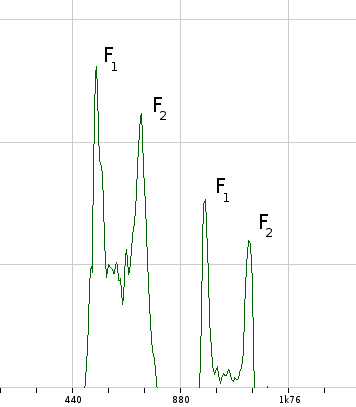
\includegraphics[width=4cm]{./png/FSK-Analysis.png}
 \caption{Zwei schmalbandige FSK-Signale, Spektrumanalyse}
 \label{fig:fsk}
\end{figure}

Bei MFSK \textit{(Multiple Frequency Shift Keying)} wird zwischen mehreren verschiedenen Frequenzen umgetastet. MFSK wird zum Beispiel bei Olivia benutzt.

\begin{figure}[h!]
 \centering
 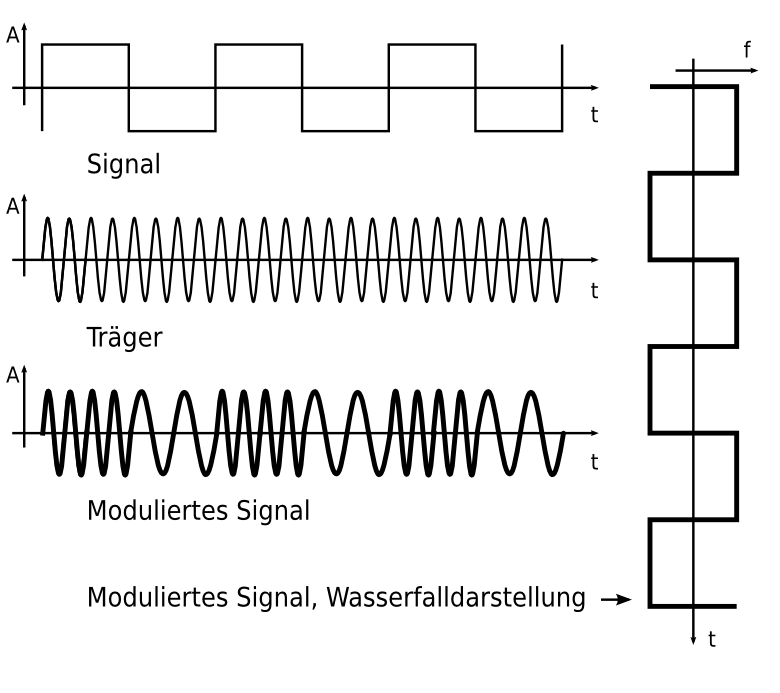
\includegraphics[width=8cm]{./png/Amfu-FSK.png}
 \caption{Modulation eines digitalen Signals (0 und 1). Die Amplitude wird im Wasserfalldiagramm wieder sichtbar.}
 \label{fig:fskMod}
\end{figure}


\subsection{PM}
Bei der Phasenmodulation wird auf die Phase eingewirkt. Eine vereinfachte Form ist das Binary Phase Shift Keying (BPSK), bei dem zwischen zwei Zuständen (0 und 1) gewechselt wird. Beim Wechsel wird die Phase um 180° gedreht, d. h. die Sinuskurve wird um eine halbe Schwingung ($\pi$) verschoben. Phasenmodulation wird für analoge Übertragungen kaum eingesetzt, eignet sich für Digitales sehr gut.

\begin{figure}[h!]
 \centering
 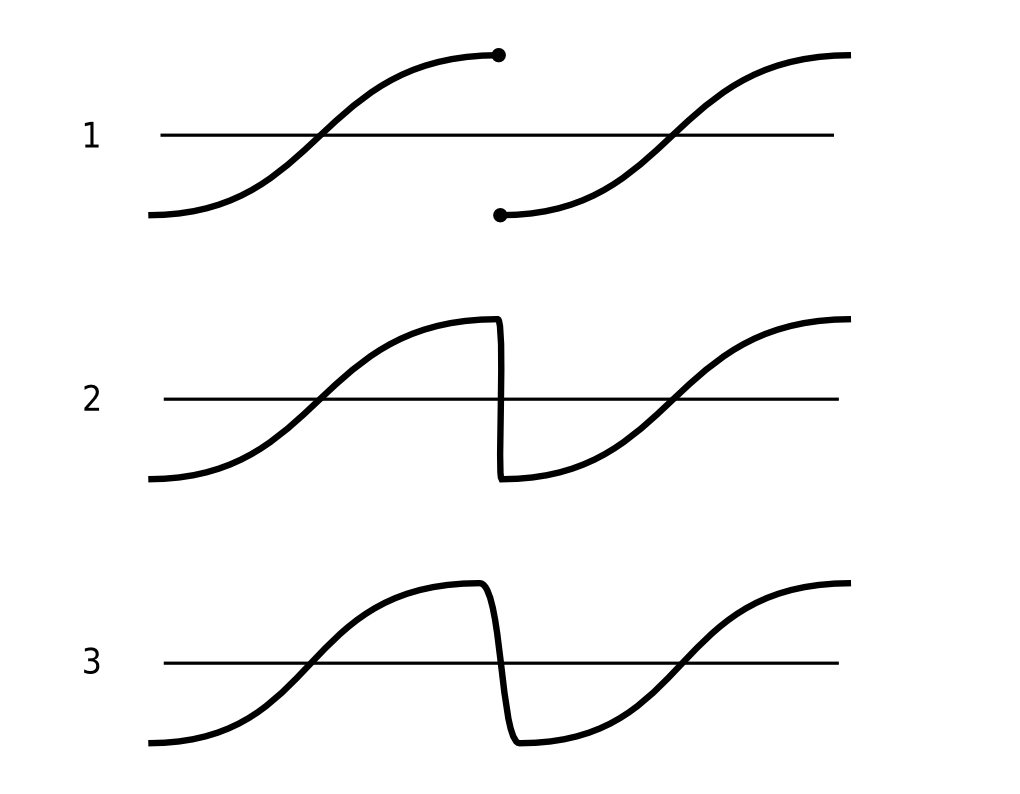
\includegraphics[width=6cm]{./png/Amfu-PM.png}
 \caption{Phasenmodulation: Phasenwechsel um 180°}
 \label{fig:pm}
\end{figure}

\begin{figure}[h!]
 \centering
 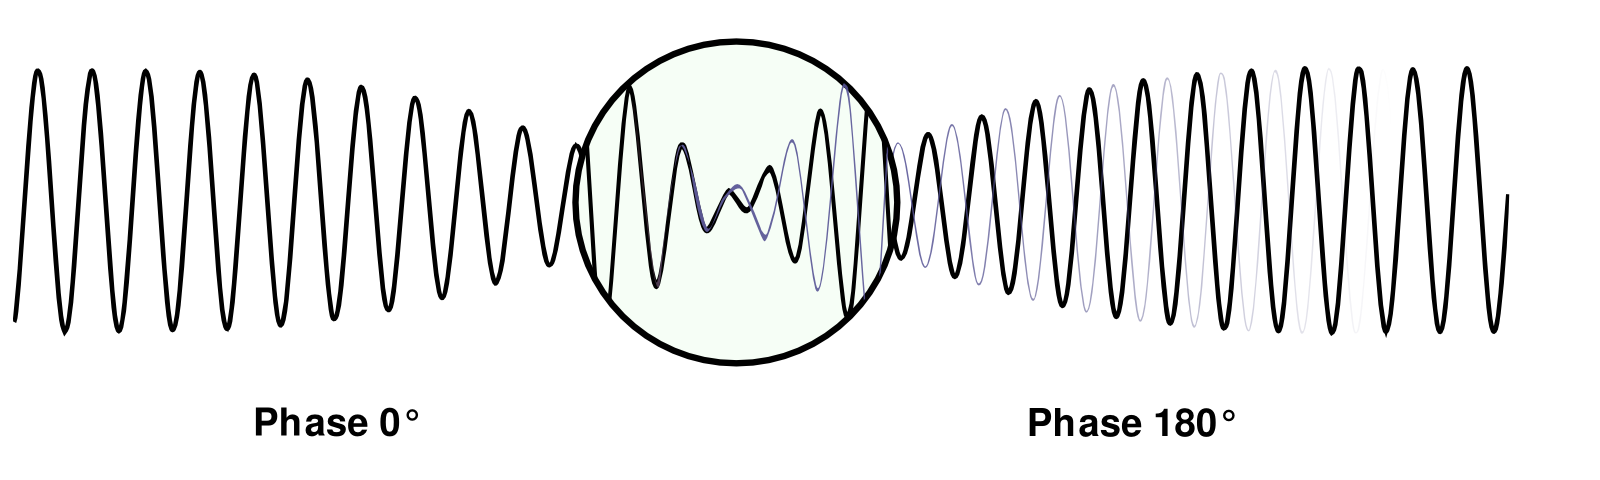
\includegraphics[width=10cm]{./png/Amfu-PSK.png}
 \caption{PSK: Die Phase wird um 180° gedreht}
 \label{fig:psk}
\end{figure}

Beim Phasenwechsel (in \link{Grafik 10 oben} um 180°) entsteht während dem Phasenwechsel für kurze Zeit eine höhere Frequenz (und somit eine höhere Bandbreite), da die beiden Punkte verbunden werden müssen (1). Eine senkrechte Verbindung würde aber zu einer sehr hohen Frequenz führen (2). Möglich wäre zum Beispiel die Kurve 3, die sich durch den Widerstand von Kabel etc. (steigt mit höherer Frequenz) automatisch ergibt. Bei PSK31 wird das Signal beim Übergang zusätzlich noch abgeschwächt.